\documentclass[tikz,border=4pt]{standalone}
\usepackage{amsmath}
\usetikzlibrary{decorations.markings}
\begin{document}
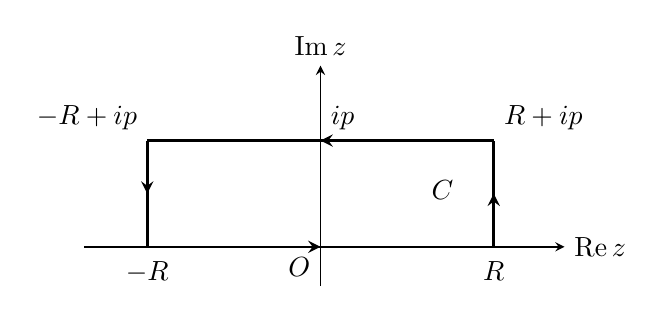
\begin{tikzpicture}[>=stealth, thick, scale=1.0]
  % Axes
  \draw[->, line width=0.5pt] (-3.0, 0) -- (3.1, 0) node[right] {$\mathrm{Re}\,z$};
  \draw[->, line width=0.5pt] (0, -0.5) -- (0, 2.3) node[above] {$\mathrm{Im}\,z$};
  \node[below left] at (0, 0) {$O$};

  % Rectangular contour C: -R -> R -> R+ip -> -R+ip -> -R
  \begin{scope}[decoration={markings, mark=at position 0.5 with {\arrow{>}}}]
    \draw[line width=0.95pt, postaction={decorate}] (-2.2, 0) -- (2.2, 0);
    \draw[line width=0.95pt, postaction={decorate}] (2.2, 0) -- (2.2, 1.35);
    \draw[line width=0.95pt, postaction={decorate}] (2.2, 1.35) -- (-2.2, 1.35);
    \draw[line width=0.95pt, postaction={decorate}] (-2.2, 1.35) -- (-2.2, 0);
  \end{scope}

  % Vertex labels
  \node[below] at (-2.2, -0.05) {$-R$};
  \node[below] at (2.2, -0.05) {$R$};
  \node[above right] at (2.2, 1.35) {$R + ip$};
  \node[above left] at (-2.2, 1.35) {$-R + ip$};
  \node[above right] at (0, 1.35) {$ip$};

  % Contour label
  \node at (1.55, 0.72) {$C$};
\end{tikzpicture}
\end{document}
